\section{Интуиционистское исчисление высказываний}
\begin{enumerate}
    \item (1 балл) Допишите указание истинности переменных в следующей шкале Крипке так,
    чтобы она опровергала формулу $(p \rightarrow q \lor r) \rightarrow (p \rightarrow q) \lor (p \rightarrow r)$:
    \begin{center}
        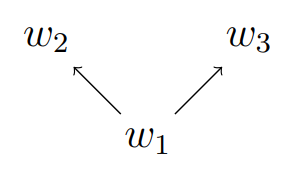
\includegraphics[width=0.15\textwidth]{hw05_1.png}
    \end{center}
    \item (1 балл) Допишите указание истинности переменных в следующей шкале Крипке так,
    чтобы она опровергала формулу $(\overline{p} \rightarrow q \lor r) \rightarrow (\overline{p} \rightarrow q) \lor (\overline{p} \rightarrow r)$:
    \begin{center}
        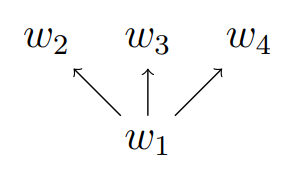
\includegraphics[width=0.15\textwidth]{hw05_2.png}
    \end{center}
    \item Постройте шкалы Крипке, опровергающие следующие формулы:
    \begin{itemize}
        \item[(a)] (1 балл) $(p \rightarrow q) \rightarrow \overline{p} \lor q$
        \item[(b)] (2 балл) $((p \rightarrow q) \rightarrow p) \rightarrow p$
    \end{itemize}
\end{enumerate}
\clearpage
